\section{Text Quality}
\label{sec:textquality}

When first approaching the topic of measuring the quality
of contributions made by users, our thinking (perhaps shaped
by some of the public discussion surrounding
contributions~\cite{Swartz2006} \mynote{Other references?})
focused on the text being added by users.
The basic assumption of a reputation system is that past performance
is a reliable indicator of future performance, so we were
asking the question ``does text added by some users \intro{survive}
longer than text by other users?''
To answer this question, we needed to track the authorship of
units of text, and then compute how much of the original text
survives into later versions of an article.
For the WikiTrust project, we opted to use a granularity of words
to reduce the computational requirements.

\subsection{Text Survival}

In Chapter~\ref{ch:diff}, we describe how to track text authorship
for the text in an article $\article{} \in \articles$.
Just tracking authorship isn't enough for tracking survival, since
we need to know what specific revision a word came from.
Let us define another recursive relation, like the definition
for $\txtauthor{}$ in Equation~\ref{eq:txtauthor},
which defines the revision that a word was first introduced.
As before, we recall
$\words{\version{n}} = \left[ w_1, w_2, \ldots, w_{l_n} \right]$, and let $0 < j \le l_n$ in the following definitions:
\begin{equation*}
\txtsrcrev{\version{n}, j} =
    \begin{cases}
        \txtsrcrev{\version{k}, s}, & \text{ if }
        \match{\version{n}, j, \prevrevs{\version{n}}} = (\version{k}, s) \\
        n, & \text{ if there is no best match text. } \\
    \end{cases}
\end{equation*}
Now we can define the text survival of words to be the number of
words introduced in \version{m} that are still present in \version{n}:
\begin{equation}
\txt{\article{}}{m}{n} = \left| j \colon \txtsrcrev{\version{m},j} = m \right| \\
\end{equation}

\subsection{Text Quality}

Our goal, in the abstract, is to define some metric that we can compute for
revisions which quantifies some estimate of the \intro{quality} of the
revision.
There are many possible ways to define quality measures, which is the
subject of research on vandalism detection (see
Section~\ref{sec:vandalism-related} for background on that topic).
As an example, a simple quality measure would be the heuristic that
inappropriate words added as part of an edit would indicate that the revision
is of poor quality.

For the purposes of building a reputation system, we want a measure
which provides some insight into the community perception of the
quality of the edit.
Having defined the notion of text survival, a very simple quality measure
could be ``what fraction of the text added in a revision survives
ten revisions later?''
We discuss some variations of these quality measures in
Chapter~\ref{ch:contrib}, but present here one novel quality measure.

In trying to understand how text contributions evolve, we decided
to limit our exploration to what happens to the text over the
following ten revisions.
Many contributions follow the simplest model: they are either
removed completely right away (a revert), or they are perfectly
preserved for the following ten revisions.
Some contributions, however, are only partially preserved, and
might even be partially restored as part of their evolution.
Figure~\ref{fig-textcontr-a} gives a pictorial representation
of how some text introduced at revision \version{k} might
evolve over the next seven revisions; in this example, the
figure shows that some text was restored in revision \version{j}.
We say that author $A_j$ \intro{judges} the work of author
$A_k$ by deciding how much text to preserve, delete, and restore.
If author $A_j$ works on a different part of the article, they
are still implicitly deciding that the current revision of
$A_k$'s work is okay; some model of user attention would be
useful for tempering the amount of judgement we infer from
$A_k$ when they are focused elsewhere in the article.

Measuring the fraction of text that survives to revision \version{j}
(\eg computing $T_j / T_k$ according to the figure)
gives useful information, but what if \version{j} happens to be
a vandal that blanks the page?
Noting that text which will be deleted is often deleted right away,
we decided to adopt a model where a contribution \intro{decays}
to its final value in an exponential fashion.


\mynote{Experiment: collect data for several different revisions.
Compute the decay for each one, and then compute the error from
the decay.  What are the statistics for this decay?}

\mynote{Can we run this experiment?}

\mynote{Need to add description of truncated Newton's method for solving
the exponential equation.}


\begin{figure}[t]
\centering
\subfigure[Graphical representation of the \textit{text survival} over
    several subsequent revisions.]{
\label{fig-textcontr-a} 
\framebox{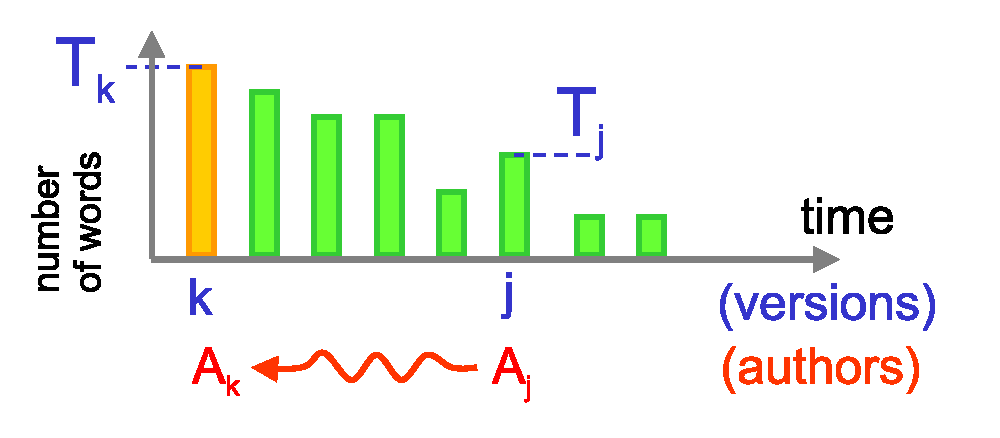
\includegraphics[width=0.9\textwidth]{part-F70-editquality/textcontr-2}}
}
\hspace{1ex}
\subfigure[Calculating the \textit{text longevity} of a contribution.]{
\label{fig-textcontr-b}
\framebox{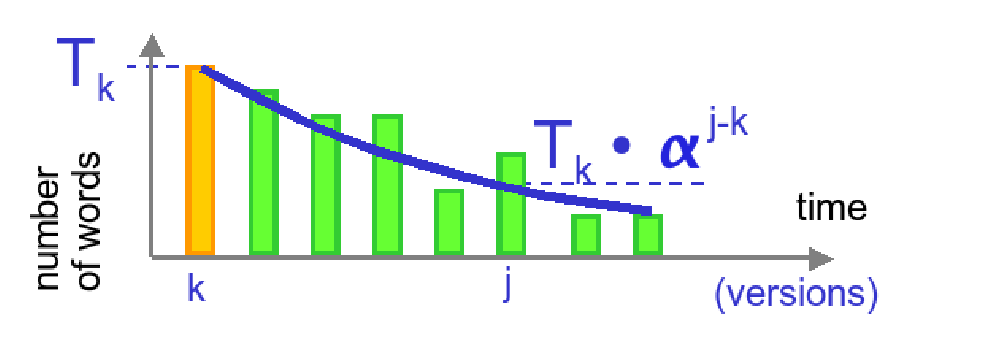
\includegraphics[width=0.9\textwidth]{part-F70-editquality/text-longevity}}
}
\caption{A graphical depiction of how a text contribution survives
	through future revisions.
	An author, \editor{k}, adds $T_k$ words in version \version{k}.
	In subsequent versions, only a portion of the words survive.
	We model the survival over time as a geometric curve,
	to arrive at a single number describing the longevity
	of the initial contribution.}
\label{fig-textsurvival}
\end{figure}


  To measure the overall quality of a single text contribution
  (see Figure~\ref{fig-textcontr-b}), we model the sequence of
  words preserved over time as a geometric curve; we call the
  value which describes the curve
  the text longevity, \tlong, of a text contribution at \revision{k}.
  Specifically, we solve the following equation for $\tlong(\revision{k})$:
  \begin{equation*}
  	\sum_{i=k+1}^n T_i = T_k \cdot
		\sum_{i=k}^n \{ \tlong(\revision{k}) \}^{i-k}
  \end{equation*}
  This value ranges from zero for a contribution which is immediately
  reverted, to one for a text contribution which is never modified.
  The intuition behind a geometric model is that if an edit is
  ``bad,'' then most of the text will be removed right away.
  As time passes, the size of the edits gets smaller and
  the text tends to stabilize into a form
  that people can agree on, until it eventually no longer changes.

